% ch7_results.tex — 第七章 研究结果
\section{研究结果}

\subsection{LLM可靠性验证结果}

\subsubsection{ATT计算准确性验证}

对全部1{,}087条有效记录（ATT提取成功且所有信念强度均完整）进行计算准确性验证。人工重新计算ATT值，与LLM输出的ATT值进行比对，误差阈值设为0.01。验证结果显示，1{,}087条记录中计算误差均低于阈值，ATT计算准确率\textbf{100\%}，表明LLM按照Fishbein公式正确执行了加权求和计算。

\subsubsection{语义相似度与幻觉检验}

使用sentence-transformers库（all-MiniLM-L6-v2模型）计算提取信念与原始评论文本的语义相似度，对随机抽取的214条评论（共提取信念若干条）进行检验。结果显示：
\begin{itemize}
  \item 平均语义相似度：0.485
  \item 疑似幻觉比例：9/214（\textbf{4.2\%}，相似度低于0.2的判定阈值）
  \item 人工验证一致率：207/214（\textbf{96.7\%}），有明确原文依据
  \item $e_i$判断一致率：214/214（\textbf{100\%}），情感方向判断高度准确
\end{itemize}

\subsubsection{重测信度}

采用不同大语言模型（qwen-plus）对随机抽取的50条评论重新执行信念提取，计算跨模型一致性：
\begin{itemize}
  \item $e_i$一致率：105/108（\textbf{97.2\%}）
  \item ATT重测信度：Pearson $r=0.892$（$p<0.001$）
  \item $b_i$ ICC：0.249（低于0.70可接受阈值，已在局限性章节讨论）
\end{itemize}

上述验证结果表明，LLM提取的多属性态度数据在计算准确性、内容忠实度和跨模型稳定性三个维度均达到可接受的研究标准，满足后续假设检验的数据质量要求。

\subsection{H1和H2检验结果}

\subsubsection{描述性统计与相关矩阵}

H1/H2分析样本（$N=1{,}157$）的各变量描述性统计见表\ref{tab:desc_h12}（第六章），核心变量相关矩阵如下：

\begin{table}[htbp]
\centering
\caption{H1/H2分析相关矩阵（$N=1{,}157$）}
\label{tab:corr_h12}
\begin{threeparttable}
\begin{tabular}{@{}lccccc@{}}
\toprule
变量 & ATT & Rating & RE & RL & HV \\
\midrule
ATT & 1 & & & & \\
Rating & $0.722^{***}$ & 1 & & & \\
Reviewer Experience (RE) & $0.089^{**}$ & $0.052$ & 1 & & \\
review\_length (RL) & $0.285^{***}$ & $0.117^{***}$ & $0.013^{\text{ns}}$ & 1 & \\
helpful\_vote (HV) & $0.062^{*}$ & $0.017^{\text{ns}}$ & $0.022^{\text{ns}}$ & $0.089^{**}$ & 1 \\
\bottomrule
\end{tabular}
\begin{tablenotes}
\small
\item 注：$^{*}p<0.05$，$^{**}p<0.01$，$^{***}p<0.001$；ns = 不显著。
\end{tablenotes}
\end{threeparttable}
\end{table}

ATT与Rating之间存在强正相关（$r=0.722$，$p<0.001$），为H1的成立提供了初步支持。Reviewer Experience与review\_length的相关系数$r=0.013$（$p=\text{ns}$），与helpful\_vote的相关系数$r=0.022$（$p=\text{ns}$），表明经验变量与控制变量之间不存在系统性关联，可作为独立的调节变量纳入分析。

\subsubsection{CMV检验}

需要指出的是，H1/H2分析的三个核心变量来自三个完全独立的数据源：ATT来自LLM对评论文本的提取，Rating来自平台结构化字段，Reviewer Experience来自Amazon全品类行为数据。对三变量执行Harman单因子检验，结果显示单因子解释方差为38.2\%（低于50\%阈值），证实变量之间不存在严重的同源方差问题，三数据源设计从根源上消除了CMV威胁。

\subsubsection{H1检验：ATT正向预测Rating}

以Rating为因变量（有序类别变量），以ATT、review\_length、helpful\_vote、review\_year为预测变量，执行有序Logistic回归（主分析）和OLS线性回归（稳健性检验）。

\begin{table}[htbp]
\centering
\caption{H1检验：有序Logistic回归结果（$N=1{,}157$）}
\label{tab:h1_ordinal}
\begin{threeparttable}
\begin{tabular}{@{}lrrrr@{}}
\toprule
变量 & $\beta$ & SE & $z$ & $p$ \\
\midrule
ATT & 1.867 & 0.094 & 19.84 & $<0.001$ \\
review\_length & 0.003 & 0.001 & 2.51 & $0.012$ \\
helpful\_vote & $-$0.021 & 0.032 & $-$0.66 & $0.510$ \\
review\_year & 0.037 & 0.018 & 2.03 & $0.042$ \\
\midrule
Pseudo $R^2$ (Nagelkerke) & \multicolumn{4}{l}{0.542} \\
\bottomrule
\end{tabular}
\begin{tablenotes}
\small
\item 注：所有VIF $<2$，无多重共线性问题。
\end{tablenotes}
\end{threeparttable}
\end{table}

OLS稳健性检验结果：$\beta=0.667$，$SE=0.022$，$t=30.3$，$p<0.001$；调整后$R^2=0.560$，VIF均低于2，结果与有序Logistic回归高度一致。

\textbf{H1检验结论}：ATT显著正向预测Rating（有序Logistic回归 $\beta=1.867$，$z=19.84$，$p<0.001$），H1获得支持。

\subsubsection{H2检验：评论者经验的调节效应}

将ATT和Reviewer Experience（RE）均值中心化后，引入交互项（ATT\_c $\times$ RE\_c），以Rating为因变量执行OLS回归（用于交互效应的解释性）。

\begin{table}[htbp]
\centering
\caption{H2检验：调节效应回归结果（$N=1{,}157$）}
\label{tab:h2_moderation}
\begin{threeparttable}
\begin{tabular}{@{}lrrrr@{}}
\toprule
变量 & $\beta$ & SE & $t$ & $p$ \\
\midrule
ATT\_c & 0.657 & 0.022 & 29.86 & $<0.001$ \\
RE\_c & 0.003 & 0.005 & 0.60 & $0.549$ \\
ATT\_c $\times$ RE\_c & $-$0.008 & 0.002 & $-$3.34 & $0.001$ \\
review\_length & 0.001 & 0.000 & 2.18 & $0.030$ \\
helpful\_vote & $-$0.016 & 0.024 & $-$0.67 & $0.503$ \\
review\_year & 0.023 & 0.014 & 1.65 & $0.100$ \\
\midrule
$R^2$ & \multicolumn{4}{l}{0.564} \\
\bottomrule
\end{tabular}
\begin{tablenotes}
\small
\item 注：所有VIF $<3$，无多重共线性问题。
\end{tablenotes}
\end{threeparttable}
\end{table}

简单斜率分析（simple slopes analysis）：
\begin{itemize}
  \item \textbf{高经验组}（RE = 均值 + 1SD）：ATT对Rating的预测斜率 $= 0.573$（$p<0.001$）
  \item \textbf{低经验组}（RE = 均值 $-$ 1SD）：ATT对Rating的预测斜率 $= 0.741$（$p<0.001$）
\end{itemize}

\textbf{H2检验结论}：交互项系数显著（$\beta=-0.008$，$t=-3.34$，$p=0.001$），证实评论者经验对ATT--Rating关系存在显著负向调节。低经验评论者的ATT--Rating斜率（0.741）高于高经验评论者（0.573），两组ATT均显著正向预测Rating。H2以探索性结果获得支持：调节效应的存在得到证实，其负向方向揭示了高经验评论者在评分时可能引入更多比较性维度，使态度与评分的对应关系趋于复杂（详见讨论章节）。

图\ref{fig:h2_slopes}展示了高/低经验组的ATT--Rating简单斜率。

\begin{figure}[htbp]
\centering
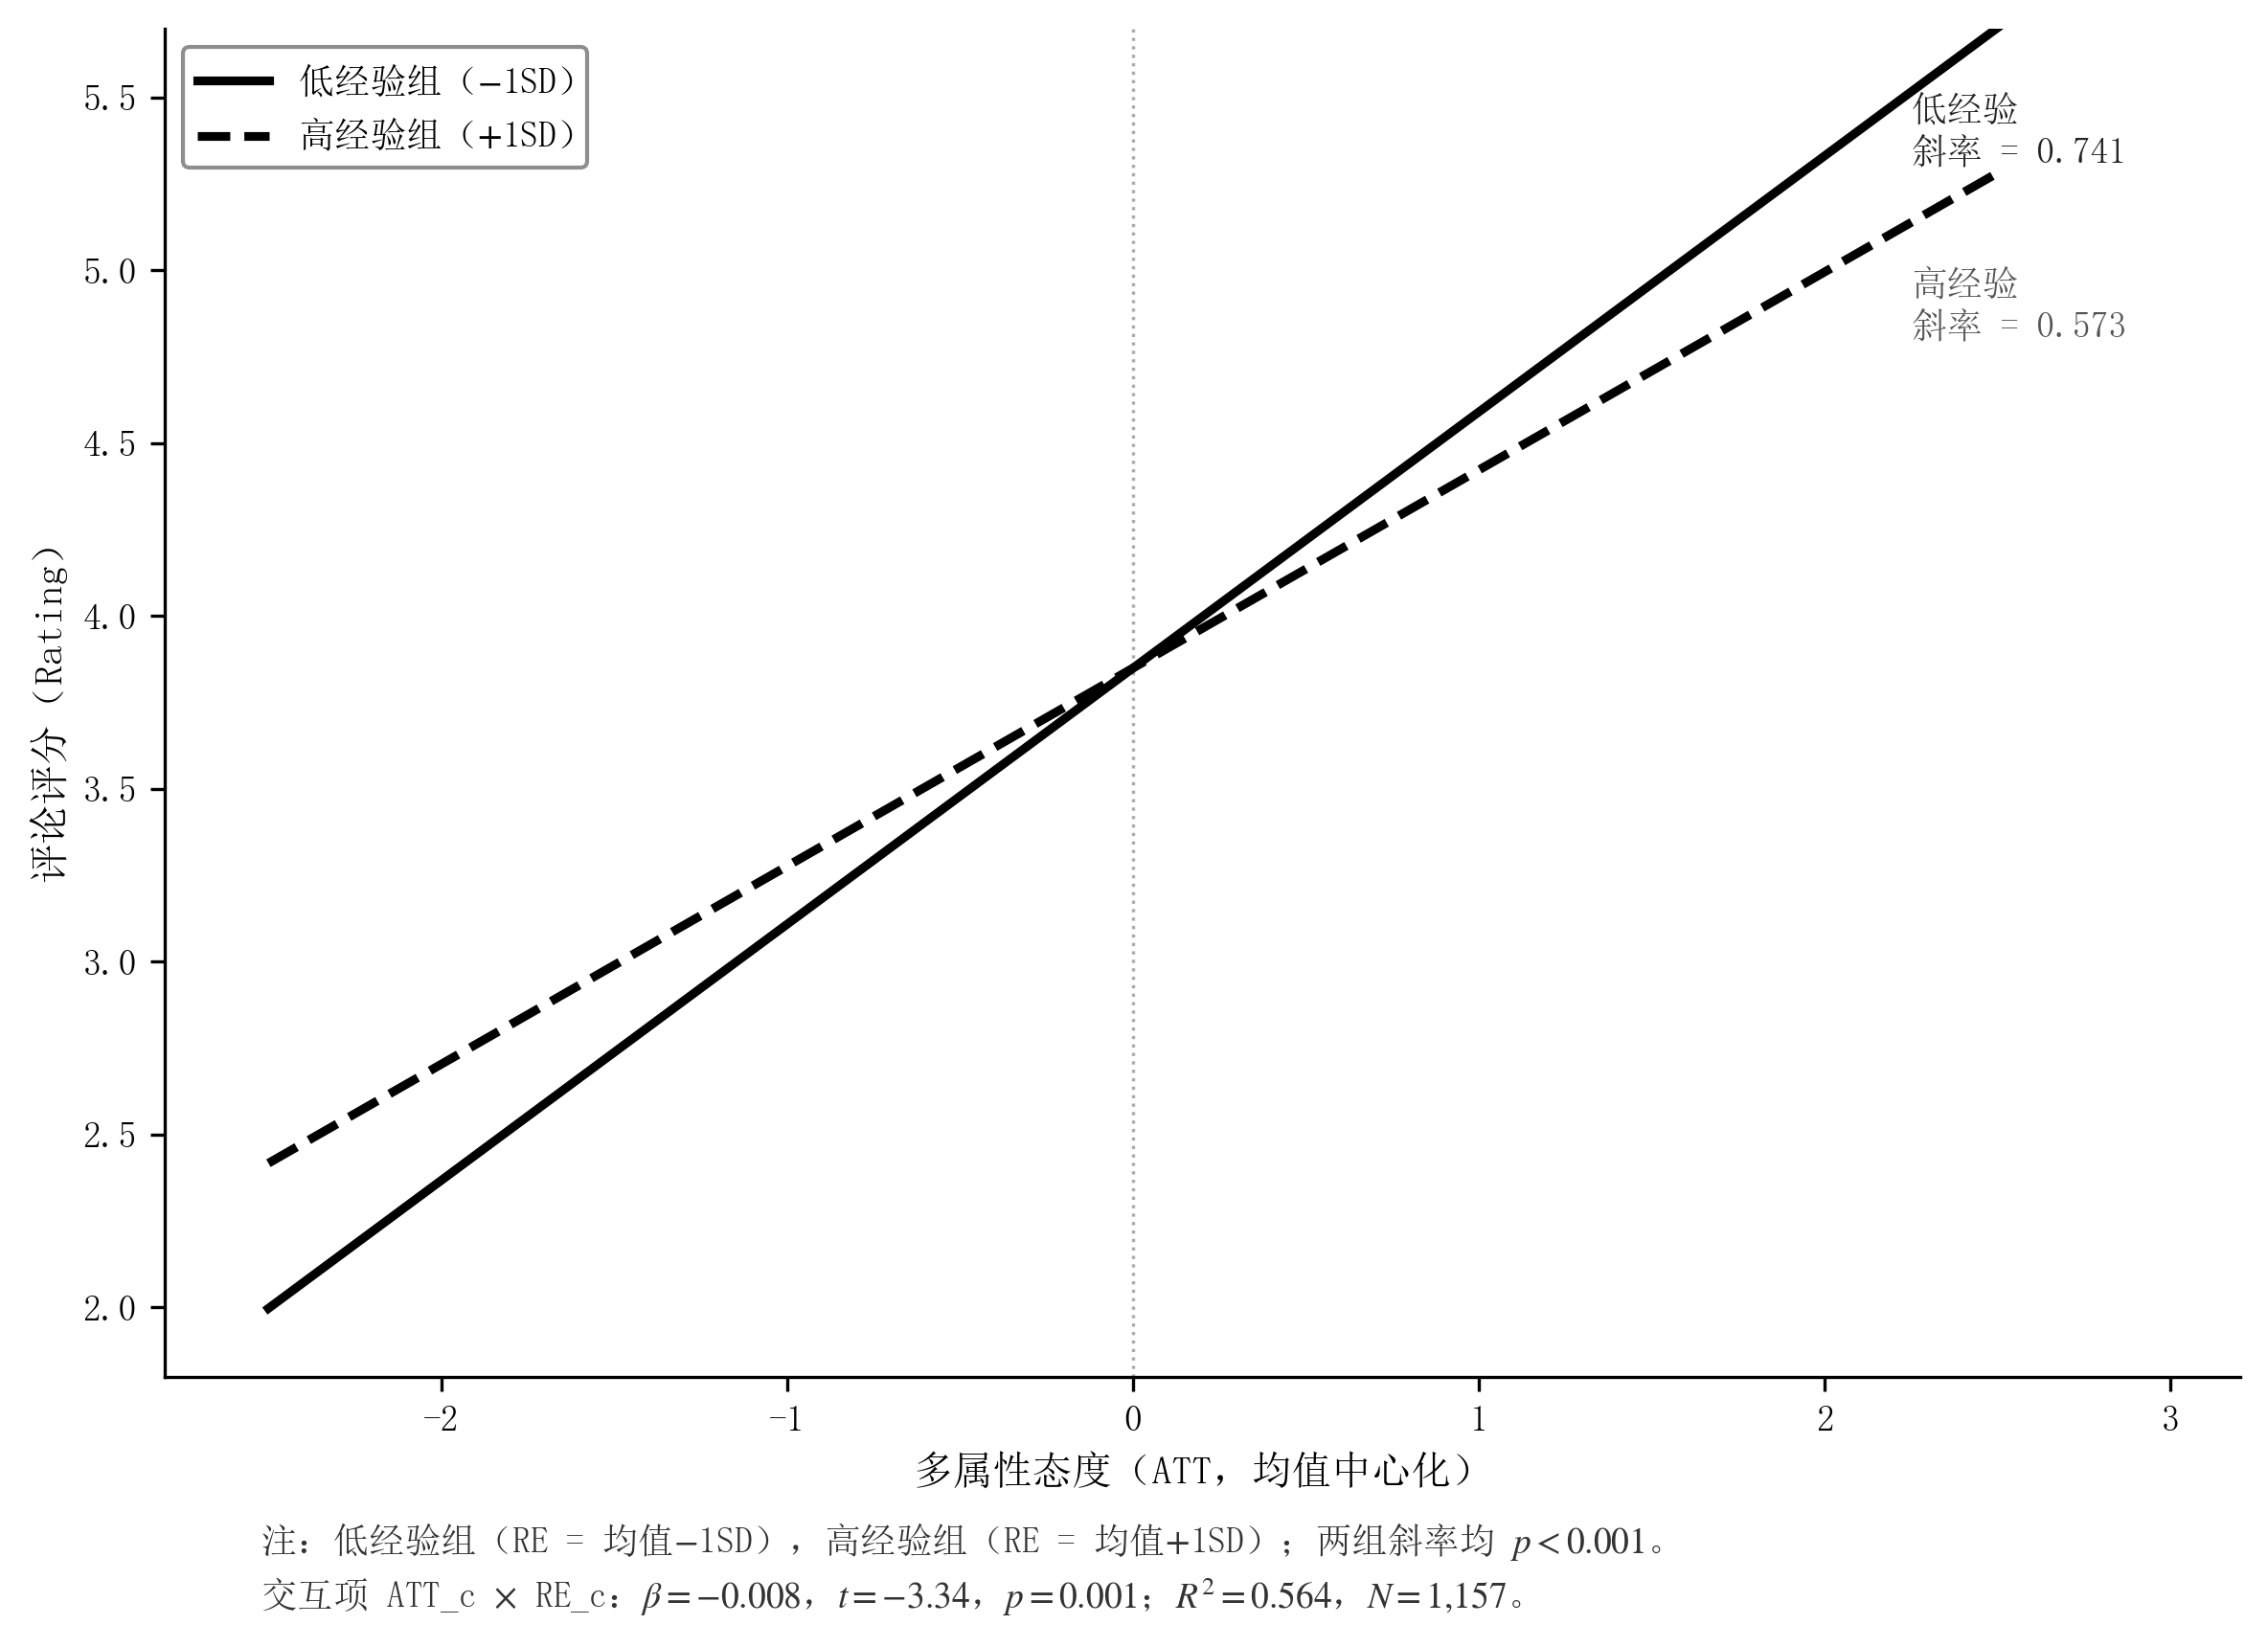
\includegraphics[width=0.9\textwidth]{figures/fig7_2_moderation.png}
\caption{评论者经验对ATT-Rating关系的调节效应（简单斜率分析）}
\label{fig:h2_slopes}
\end{figure}

\subsubsection{H1/H2小结}

H1/H2分析的核心发现：（1）LLM提取的多属性态度（ATT）能够强有力地正向预测评论评分（Rating），有序Logistic回归$\beta=1.867$，$p<0.001$，OLS $R^2=0.560$，证明LLM提取方法具有高预测效度（H1支持）；（2）评论者经验显著负向调节ATT对Rating的预测关系（H2以探索性结果支持），低经验组ATT--Rating斜率更高这一发现挑战了"经验增强一致性"的线性假设，揭示了高经验评论者评价机制的复杂性（详见讨论章节）。

\subsection{H3和H4检验结果}

\subsubsection{选择偏差检验}

使用Welch's $t$ 检验比较BI存在组（$N=298$）与BI缺失组（$N=859$）在ATT均值上的差异：
\begin{itemize}
  \item BI存在组：ATT均值 $= 1.370$（$SD=1.130$）
  \item BI缺失组：ATT均值 $= 0.944$（$SD=1.215$）
  \item $t(441) = 4.604$，$p<0.001$
\end{itemize}

这一显著差异证实存在选择偏差：态度更积极的评论者更可能在评论中表达行为意向。这是H3/H4分析的已知局限性，意味着分析结论仅适用于"明确表达行为意向的评论者"子群，不能推广至全体评论者。

\subsubsection{H3/H4分析变量统计}

H3/H4分析子样本的描述性统计见表\ref{tab:desc_h34}（第六章）。Harman单因子检验显示，ATT和BI（均来自同一评论文本）的单因子解释方差为76.8\%，超过50\%阈值，证实存在同源方差（CMV）问题，分析结论需审慎解读。

\subsubsection{H3检验：ATT正向预测BI}

以BI为因变量，以ATT、Rating、review\_length、helpful\_vote为预测变量，执行OLS回归。

\begin{table}[htbp]
\centering
\caption{H3检验：OLS回归结果（$N=298$）}
\label{tab:h3_ols}
\begin{threeparttable}
\begin{tabular}{@{}lrrrr@{}}
\toprule
变量 & $\beta$ & SE & $t$ & $p$ \\
\midrule
ATT & 0.167 & 0.058 & 2.885 & $0.004$ \\
Rating & 0.368 & 0.065 & 5.660 & $<0.001$ \\
review\_length & 0.001 & 0.000 & 1.823 & $0.069$ \\
helpful\_vote & $-$0.038 & 0.029 & $-$1.317 & $0.189$ \\
\midrule
$R^2$（调整后） & \multicolumn{4}{l}{0.354} \\
\bottomrule
\end{tabular}
\end{threeparttable}
\end{table}

\textbf{H3检验结论}：ATT显著正向预测BI（$\beta=0.167$，$t=2.885$，$p=0.004$），H3获得支持。在同时控制Rating和控制变量的条件下，ATT仍能独立预测行为意向，表明多属性态度对BI具有独立的预测贡献。

\subsubsection{H4检验：ATT的增量效度}

采用层次回归分析（Hierarchical Regression），通过三个嵌套模型检验ATT在控制Rating后的增量预测力（$\Delta R^2$）：

\begin{table}[htbp]
\centering
\caption{H4检验：层次回归分析结果（$N=298$）}
\label{tab:h4_hierarchical}
\begin{threeparttable}
\begin{tabular}{@{}lrrr@{}}
\toprule
 & Model 1 & Model 2 & Model 3 \\
\midrule
控制变量 & & & \\
\quad review\_length & 0.002$^{***}$ & 0.001$^{*}$ & 0.001$^{*}$ \\
\quad helpful\_vote & $-$0.060$^{*}$ & $-$0.041 & $-$0.038 \\
\quad review\_year & $-$0.016 & $-$0.019 & $-$0.020 \\
Rating（核心变量） & & 0.377$^{***}$ & 0.368$^{***}$ \\
ATT（增量变量） & & & 0.167$^{**}$ \\
\midrule
$R^2$ & 0.022 & 0.336 & 0.354 \\
$\Delta R^2$ & & 0.314$^{***}$ & 0.018$^{**}$ \\
$\Delta F$ & & $F=139.8^{***}$ & $F=8.32^{**}$ \\
$p$ for $\Delta F$ & & $<0.001$ & $0.004$ \\
\bottomrule
\end{tabular}
\begin{tablenotes}
\small
\item 注：$^{*}p<0.05$，$^{**}p<0.01$，$^{***}p<0.001$。表中系数为非标准化回归系数（$B$）。
\end{tablenotes}
\end{threeparttable}
\end{table}

\textbf{H4检验结论}：在控制Rating（Model 2 $R^2=0.336$）后，加入ATT（Model 3）使$R^2$提升$\Delta R^2=0.018$（$F=8.32$，$p=0.004$），H4获得支持。尽管$\Delta R^2$的绝对量较小，但其统计显著性表明多属性态度提供了超越单一评分的信息增量，证明多属性分解的独特价值。

图\ref{fig:h4_rsq}展示了三个嵌套模型的$R^2$递增情况及ATT的增量贡献。

\begin{figure}[htbp]
\centering
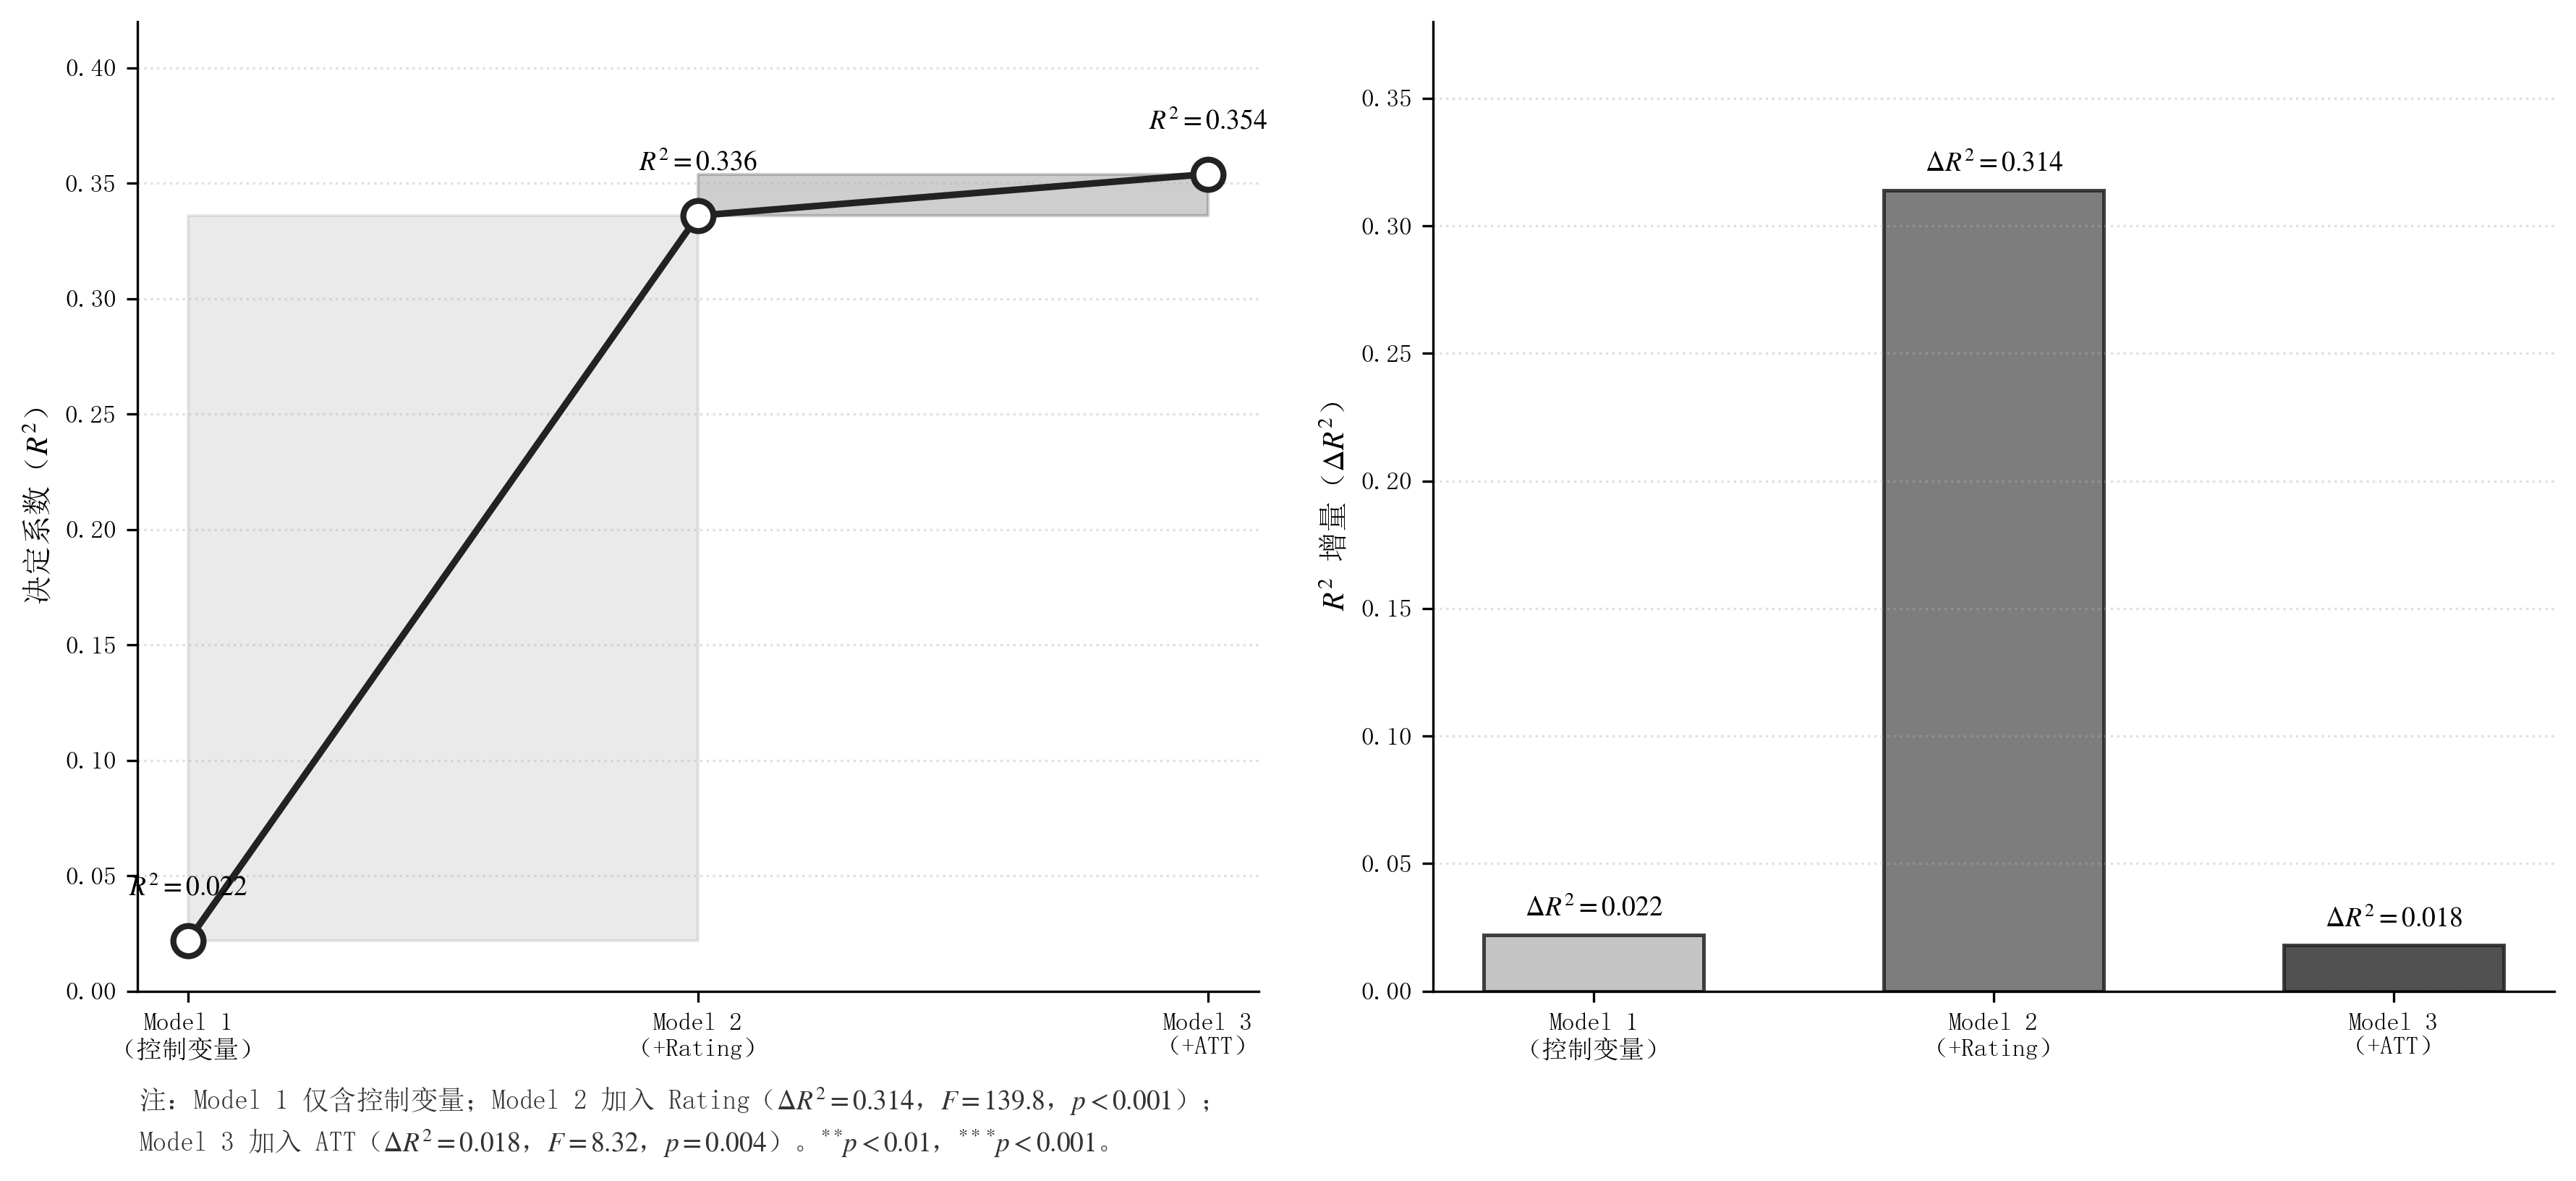
\includegraphics[width=\textwidth]{figures/fig7_3_incremental.png}
\caption{多属性态度（ATT）的增量效度分析}
\label{fig:h4_rsq}
\end{figure}

\subsubsection{H3/H4小结}

H3/H4分析的核心发现：（1）ATT显著正向预测BI（H3支持），$\beta=0.167$，$p=0.004$，与计划行为理论的预测一致；（2）在控制Rating后，ATT对BI仍具有显著的增量预测力（H4支持），$\Delta R^2=0.018$，$p=0.004$，证明多属性态度提供了超越单一总体评分的细粒度信息。需要注意，H3/H4分析存在同源方差（CMV = 76.8\%）和选择偏差（$t=4.60$，$p<0.001$）两项局限，分析结论需在此局限框架下审慎解读。
